\documentclass[aspectratio=169]{beamer}
\usetheme{Madrid}
\usecolortheme{default}

\usepackage{booktabs}
\usepackage{graphicx}
\usepackage{amsmath}
\usepackage{tikz}

\definecolor{iitmblue}{RGB}{0,47,108}
\definecolor{lightblue}{RGB}{51,122,183}

\setbeamercolor{title}{fg=white,bg=iitmblue}
\setbeamercolor{frametitle}{fg=white,bg=iitmblue}
\setbeamercolor{structure}{fg=iitmblue}

\title{DL-SIFA: Deep Learning Statistical \\Ineffective Fault Analysis on AES-128}
\subtitle{CS6630 --- Secure Processor Microarchitecture}
\author{Singh Shivam Ramdarash \\ \small CS25M048}
\institute{Indian Institute of Technology Madras}
\date{May 2026}

\begin{document}

% ======== SLIDE 1: TITLE ========
\begin{frame}
\titlepage
\end{frame}

% ======== SLIDE 2: OUTLINE ========
\begin{frame}{Outline}
\tableofcontents
\end{frame}

\section{Introduction}
\begin{frame}{Background: Fault Attacks and Defenses}
\begin{columns}[T]
\begin{column}{0.55\textwidth}
\textbf{Fault Attacks:}
\begin{itemize}
    \item Inject physical faults during encryption
    \item Faulty output leaks the secret key
    \item DFA needs both correct and faulty ciphertexts
\end{itemize}

\vspace{0.3cm}
\textbf{Defense --- Temporal Redundancy:}
\begin{itemize}
    \item Encrypt the same plaintext \textbf{twice}, compare
    \item Outputs differ $\rightarrow$ fault detected $\rightarrow$ suppress
    \item Blocks DFA completely
\end{itemize}
\end{column}
\begin{column}{0.42\textwidth}
\centering
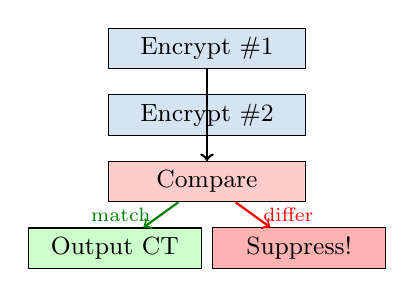
\begin{tikzpicture}[scale=0.65, every node/.style={font=\small}]
    \node[draw, fill=lightblue!20, minimum width=2.5cm] (e1) at (0,3.5) {Encrypt \#1};
    \node[draw, fill=lightblue!20, minimum width=2.5cm] (e2) at (0,2.2) {Encrypt \#2};
    \node[draw, fill=red!20, minimum width=2.5cm] (cmp) at (0,0.9) {Compare};
    \node[draw, fill=green!20, minimum width=2.2cm] (out) at (-1.8,-0.4) {Output CT};
    \node[draw, fill=red!30, minimum width=2.2cm] (sup) at (1.8,-0.4) {Suppress!};
    \draw[->,thick] (e1) -- (cmp);
    \draw[->,thick] (e2) -- (cmp);
    \draw[->,thick,green!50!black] (cmp) -- node[left,font=\scriptsize]{match} (out);
    \draw[->,thick,red] (cmp) -- node[right,font=\scriptsize]{differ} (sup);
\end{tikzpicture}
\end{column}
\end{columns}
\end{frame}

% ======== SLIDE 3: SIFA + GOAL ========
\begin{frame}{SIFA: Breaking Temporal Redundancy}
\begin{block}{Key Insight (Dobraunig et al., TCHES 2018)}
$\sim$50\% of injected faults are \textit{ineffective}---the target bit was already in the faulted state. These pass the redundancy check, but carry a \textbf{statistical bias} that leaks the key.
\end{block}

\vspace{0.3cm}
\textbf{Project Goal:}
\begin{enumerate}
    \item Implement AES-128 with temporal redundancy + stuck-at-0 faults at Round 8
    \item \textbf{Traditional SIFA}: recover key using bit-bias formula
    \item \textbf{DL-SIFA}: recover key using a trained neural network
    \item Compare trace efficiency of both methods
\end{enumerate}

\vspace{0.2cm}
\small Based on: Ramezanpour et al., \textit{``Fault Intensity Map Analysis with NN Key Distinguisher''}, ASHES 2019.
\end{frame}

\section{Fault Model}
\begin{frame}{Fault Model and Bias Mechanism}
\begin{columns}[T]
\begin{column}{0.5\textwidth}
\begin{tabular}{ll}
\toprule
Fault & Stuck-at-0 (bit 0) \\
Location & Round 8 SubBytes input \\
Attempts & 50,000 per byte \\
Ineffective rate & $\sim$50\% \\
Traces kept & $\sim$25,000 \\
\bottomrule
\end{tabular}

\vspace{0.4cm}
\textbf{Why bias?} \\
Normal: byte $\in \{0 \ldots 255\}$ (256 values) \\
After fault: only even values survive (128) \\
$\rightarrow$ half the histogram bins are empty
\end{column}
\begin{column}{0.45\textwidth}
\centering
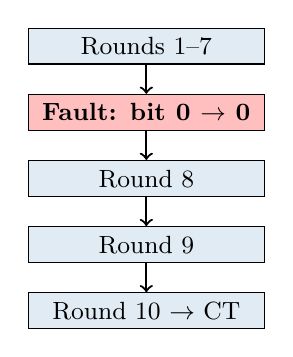
\begin{tikzpicture}[scale=0.7, every node/.style={font=\small}]
    \node[draw, fill=lightblue!15, minimum width=3cm] (r7) at (0,4.5) {Rounds 1--7};
    \node[draw, fill=red!25, minimum width=3cm] (fault) at (0,3.3) {\textbf{Fault: bit 0 $\rightarrow$ 0}};
    \node[draw, fill=lightblue!15, minimum width=3cm] (r8) at (0,2.1) {Round 8};
    \node[draw, fill=lightblue!15, minimum width=3cm] (r9) at (0,0.9) {Round 9};
    \node[draw, fill=lightblue!15, minimum width=3cm] (r10) at (0,-0.3) {Round 10 $\rightarrow$ CT};
    \draw[->,thick] (r7) -- (fault);
    \draw[->,thick] (fault) -- (r8);
    \draw[->,thick] (r8) -- (r9);
    \draw[->,thick] (r9) -- (r10);
\end{tikzpicture}
\end{column}
\end{columns}
\end{frame}

\section{Traditional SIFA}
\begin{frame}{Traditional SIFA: Bit-Bias Key Recovery}
\textbf{Algorithm}: For each key guess $k \in \{0, \ldots, 255\}$:
\begin{enumerate}
    \item Invert each CT through rounds 10, 9, 8 using guess $k$
    \item Compute bias $= \frac{\#(\text{bit 0}=0)}{N}$. \quad Correct key $\rightarrow 1.0$, \quad Wrong $\rightarrow 0.5$
\end{enumerate}

\vspace{0.2cm}
\begin{columns}[T]
\begin{column}{0.48\textwidth}
\textbf{Results:}
\begin{itemize}
    \item All 16 bytes: bias $= 1.0000$
    \item Recovered $K_{10}[0] = \texttt{0xD0}$ \checkmark
    \item Correct bias: 1.0, avg wrong: 0.498
    \item \textbf{Min traces: 20}
\end{itemize}
\end{column}
\begin{column}{0.48\textwidth}
\centering
\small \textbf{Progressive recovery:}
\vspace{0.1cm}

\begin{tabular}{cc}
\toprule
\textbf{Traces} & \textbf{Result} \\
\midrule
10 & FAIL \\
\textbf{20} & \textbf{SUCCESS} \\
50+ & SUCCESS \\
\bottomrule
\end{tabular}
\end{column}
\end{columns}
\end{frame}

\section{DL-SIFA}
\begin{frame}{DL-SIFA: Neural Network Approach}
\textbf{Motivation}: Traditional SIFA needs exact fault model. In real hardware, faults are noisy and imprecise.

\vspace{0.2cm}
\begin{columns}[T]
\begin{column}{0.48\textwidth}
\textbf{Profiling} (500 random keys):
\begin{enumerate}
    \item Collect faulted + clean CTs
    \item Invert to R8, build \textbf{256-bin histogram}
    \item Label: biased $=1$, clean $=0$
    \item 3,000 training samples
\end{enumerate}

\vspace{0.2cm}
\textbf{Attack} (unknown key):
\begin{enumerate}
    \item For each guess: invert, histogram, NN score
    \item Highest score $=$ recovered key
\end{enumerate}
\end{column}
\begin{column}{0.48\textwidth}
\textbf{MLP Architecture:}
\vspace{0.1cm}

\begin{tabular}{lcl}
\toprule
\textbf{Layer} & \textbf{Size} & \textbf{Details} \\
\midrule
Input & 256 & Histogram \\
FC+BN & 128 & ReLU, Drop 0.3 \\
FC+BN & 64 & ReLU, Drop 0.2 \\
FC & 32 & ReLU \\
Output & 1 & Sigmoid \\
\bottomrule
\end{tabular}

\vspace{0.2cm}
\small BCE loss, Adam (lr=0.001) \\
200 epochs, PyTorch
\end{column}
\end{columns}
\end{frame}

% ======== SLIDE 7: DL-SIFA RESULTS ========
\begin{frame}{DL-SIFA: Results}
\begin{columns}[T]
\begin{column}{0.48\textwidth}
\textbf{Training:} 100\% accuracy

\vspace{0.3cm}
\textbf{Key recovery:}
\begin{itemize}
    \item Recovered $K_{10}[0] = \texttt{0xD0}$ \checkmark
    \item Correct score: \textbf{1.0000}
    \item Avg wrong score: 0.0001
    \item \textbf{Min traces: 50}
\end{itemize}

\vspace{0.3cm}
\small Stronger separation than traditional: \\
1.0 vs 0.0 (instead of 1.0 vs 0.5)
\end{column}
\begin{column}{0.48\textwidth}
\centering
\small \textbf{Progressive recovery:}
\vspace{0.1cm}

\begin{tabular}{cc}
\toprule
\textbf{Traces} & \textbf{Result} \\
\midrule
10 & FAIL \\
20 & FAIL \\
\textbf{50} & \textbf{SUCCESS} \\
100+ & SUCCESS \\
\bottomrule
\end{tabular}

\vspace{0.3cm}
\small With $<$50 traces, histogram is \\
too noisy for the NN.
\end{column}
\end{columns}
\end{frame}

\section{Comparison}
\begin{frame}{Comparison: Traditional vs DL-SIFA}
\begin{center}
\begin{tabular}{lcc}
\toprule
\textbf{Criterion} & \textbf{Traditional SIFA} & \textbf{DL-SIFA} \\
\midrule
Key recovered & \checkmark (\texttt{0xD0}) & \checkmark (\texttt{0xD0}) \\
Min traces & \textbf{20} & 50 \\
Separation & 1.0 vs 0.5 & \textbf{1.0 vs 0.0} \\
Needs fault model & Yes & \textbf{No} \\
Noise tolerance & No & \textbf{Yes} \\
Complexity & Low (formula) & High (training) \\
\bottomrule
\end{tabular}
\end{center}

\vspace{0.3cm}
\begin{columns}[T]
\begin{column}{0.48\textwidth}
\textbf{Traditional}: fewer traces, simpler, but only works with known fault model
\end{column}
\begin{column}{0.48\textwidth}
\textbf{DL-SIFA}: stronger signal, works without knowing fault details, more practical for real hardware
\end{column}
\end{columns}
\end{frame}

% ======== SLIDE 9: PLOTS ========
\begin{frame}{Results}
\vspace{-0.3cm}
\begin{center}
    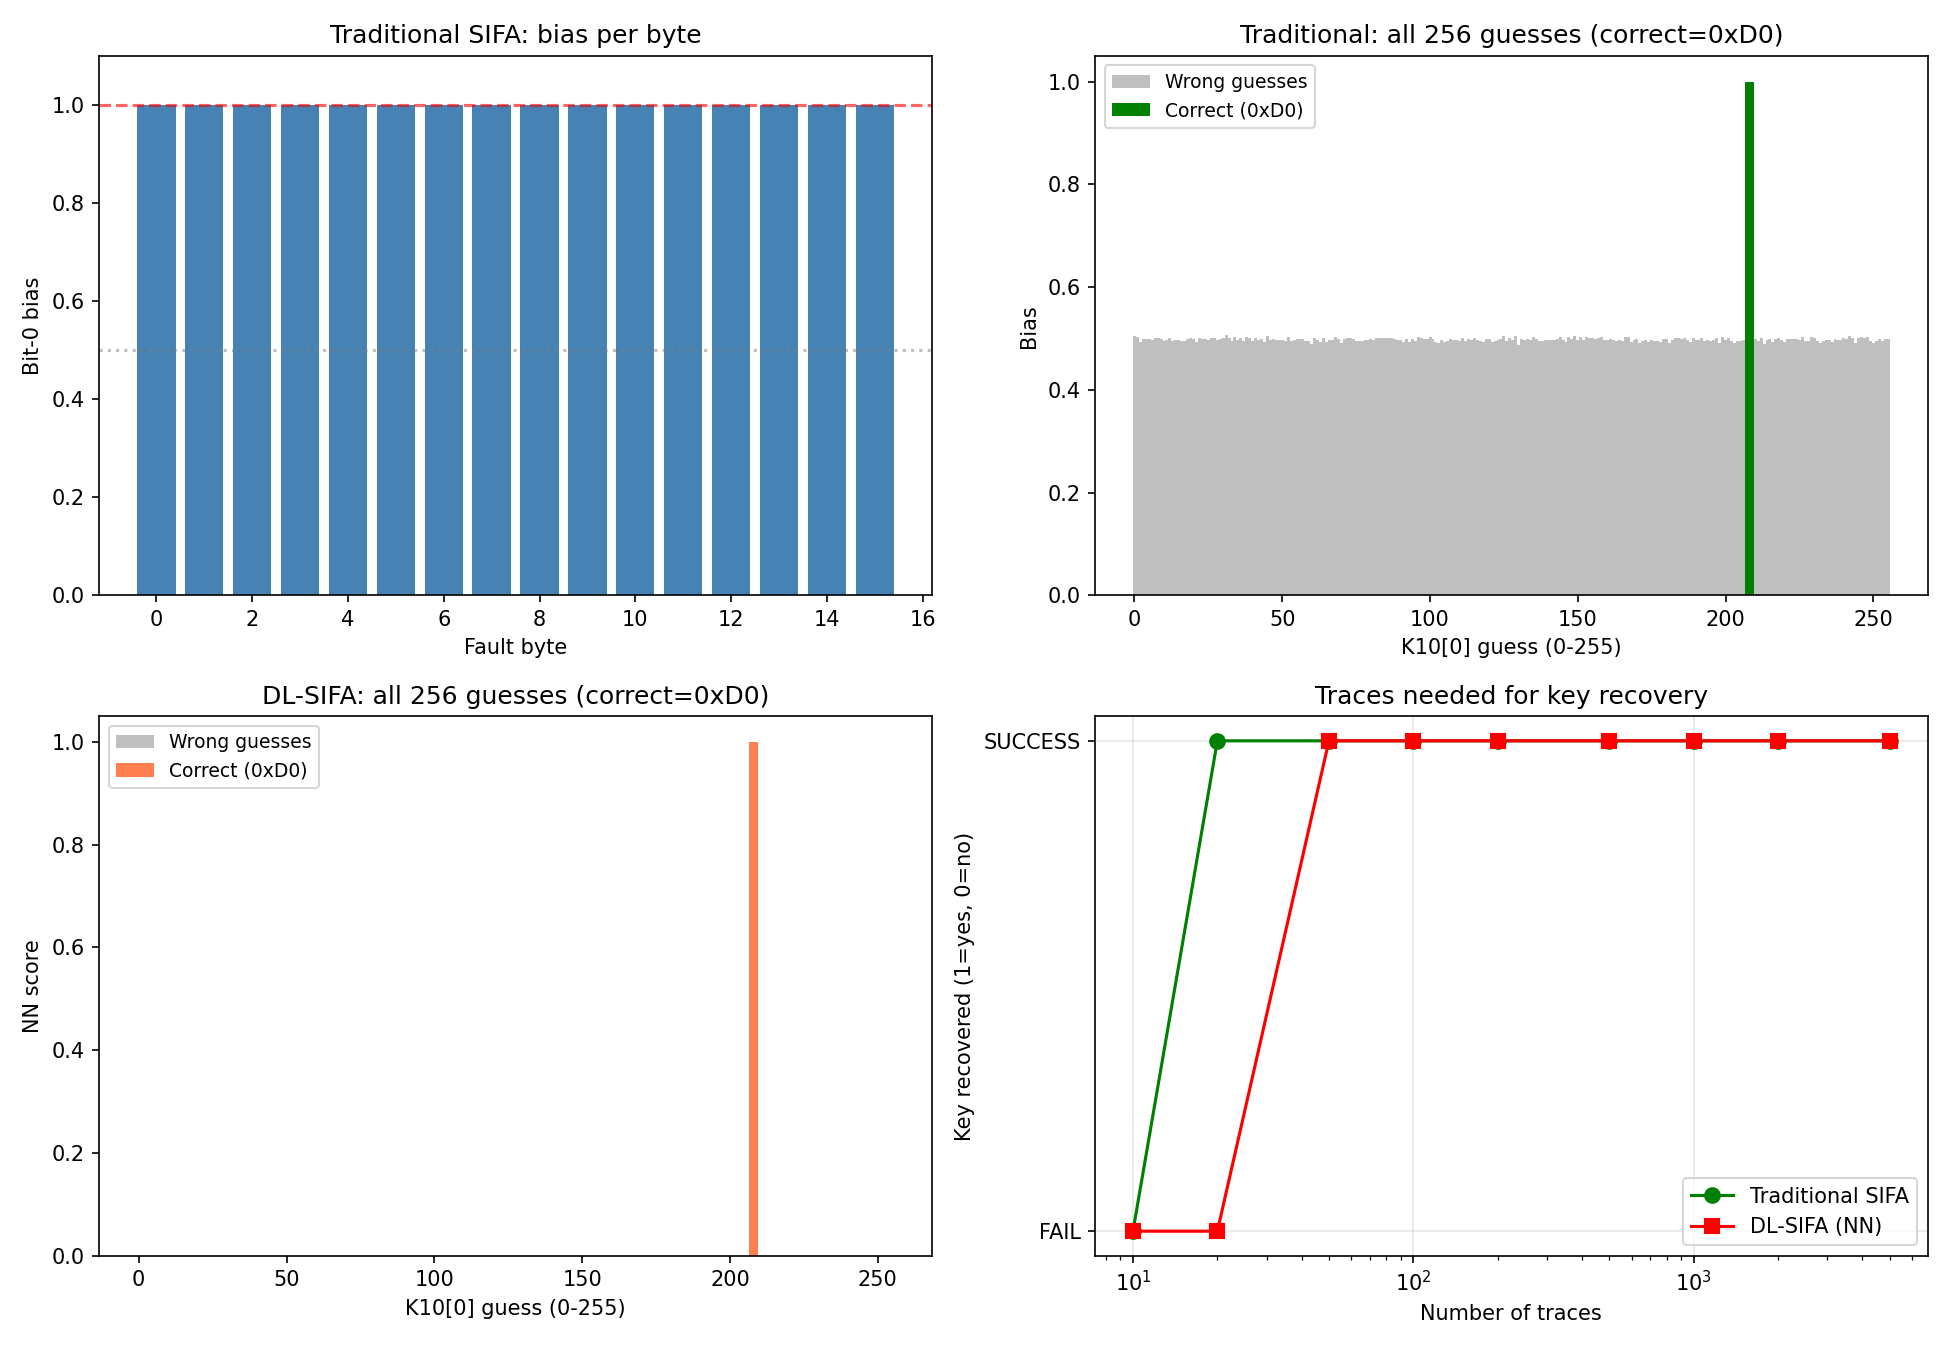
\includegraphics[width=0.78\textwidth,height=0.82\textheight,keepaspectratio]{results/comparison.png}
\end{center}
\end{frame}

\section{Conclusion}
\begin{frame}{Conclusion}
\begin{enumerate}
    \item SIFA breaks AES-128 with temporal redundancy using only \textbf{correct outputs}
    \item Both methods recover $K_{10}[0] = \texttt{0xD0}$
    \item Traditional SIFA: \textbf{20 traces}, but needs exact fault model
    \item DL-SIFA: \textbf{50 traces}, fault-model agnostic, better separation
    \item Real-world faults are rarely known precisely $\rightarrow$ DL-SIFA is more practical
\end{enumerate}

\vspace{0.3cm}
\textbf{Future work}: noisy faults, multi-bit faults, other ciphers, CNNs

\vspace{0.4cm}
\small\textbf{References:}
\begin{enumerate}\small
    \item Dobraunig et al., ``SIFA,'' TCHES 2018
    \item Ramezanpour et al., ``Fault intensity map analysis with NN key distinguisher,'' ASHES 2019
\end{enumerate}
\end{frame}

% ======== SLIDE 12: THANK YOU ========
\begin{frame}{}
\vfill
\begin{center}
\Huge \textbf{Thank You!}

\vspace{0.8cm}
\Large Questions?
\end{center}
\vfill
\end{frame}

\end{document}
